\chapter{Searching for Riders}
\label{searchForRiders}
\index{Offer!finding matching requests for given offer}
\index{Request!finding matching requests for given offer}
In this section we give a more detailled description of the \emph{"Search For Riders Algorithm"}
which finds matching requests for a given offer.
Searching for riders is done when a new offer gets created. this comprises the 
steps described in section \ref{sfrCreatingRoute} to \ref{sfrApplyingLimits}:


\section{Step 1: Create Route and Routepoints}
\label{sfrCreatingRoute}

First step when creating an offer is creating the \emph{route} associated to the offer
by calling the RouteMatchingBean.computeInitialRoutes(...) method.
\subsubsection{Routepoints}
The route is an ordered list of \emph{routepoints}. Routepoints are modelled by the 
RoutePointEntity class, which has the following main properties:
\begin{description}
     	 \item[Integer routeIdx]{Index of the routepoint inside the route (which is an ordered list of routepoints)} 
	 \item[Point coordinate]{Spatial coordinates of the routepoint in longitude/latitude form} 
  	 \item[Timestamp expectedArrival]{Date/Time when the driver is expected to reach that point}     
    	 \item[Integer seatsAvailable]{Number of free seats the driver has availlable when reaching that point} 
	 \item[Double distanceToSourceMeters]{Road distance to the startpoint in meters.} 
\end{description}

Henceforth, we may abbreviate the term $RoutePoint$ with $RP$.

\section{Step 2: Create Drive Route Points}
\label{sfrScanningTheCorridor}
As depicted in \ref{searchForRiderShort}, in order to find a preselection of matching requests,
a corridor consisting of all the points that have distance less than the driver defined maximum detour 
is scanned for start and endpoints of requests.
The task of "scanning the corridor of distance max detour" is somewhat complicated and it's 
implementation is based on an auxiliary construction named "Drive Route Points", which we discuss next.
 
\subsection{The Circle Overlay Algorithm}
\label{sfrDriveRoutePoints}
\label{sfrCircleOverlayAlgorithm}
The principal Idea is to approximate the corridor of distance $detour$ around the path by a  number of
so called \emph{Drive Route Points} (henceforth abbreviated DRPs). 
The DRPs are chosen as a subset of the set of RPs. 
Instead of testing wether or not a point $P$ is in the corridor, we test if there is a DRP  which is close enough to $P$.
Figure \ref{pic:circleOverlayAlgorithmImage} depicts the circle overlay algorithm.

	\begin{figure}[t]
	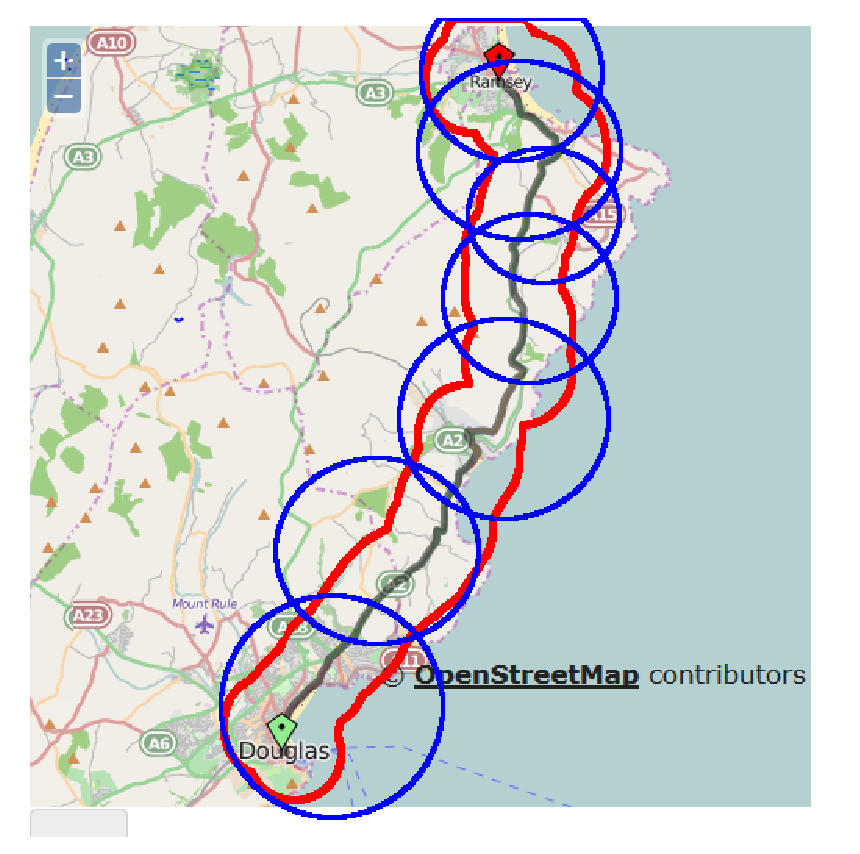
\includegraphics[scale=0.5]{images/maps_drp/02-OSM-DouglasToRamsay.corridor.eps}
	\caption{Red lines mark the exact corridor of distance $detour_{max}$ around Janet's route,
	         The blue circles are a covering of the corridor as used by the circle overlay algoritm.
		 }
	\label{pic:circleOverlayAlgorithmImage}
	\end{figure}

As the surface covered by these Circles is larger than the corridor, the circle overlay algorithm produces more false
positives as checking the exact corridor would do. However, beeing used at the preselection stage, this step 
is supposed to produce only a preliminary list of results, which may contain a number of 
false positives which are removed at subsequent stages of the search for rider algorithm.
The advantage in speed and effort of using circle overlay instead of the exact corridor anyway outweights this disadvantage.

\subsection{Drive Route Points}

In ORS, DRPs are modelled by the \emph{DriveRoutePointEntity} class.
These are the main properties of a DriveRoutePointEntity:

\begin{description}
     	 \item[Integer routeIdx]{Index of the routepoint inside ordered list of DRPs)} 
	 \item[Point coordinate]{Spatial coordinates in longitude/latitude form} 
  	 \item[Timestamp expectedArrival]{Date/Time when the driver is expected to reach that point}     
    	 \item[Integer seatsAvailable]{Number of free seats the driver has availlable when reaching that point} 
	 \item[Double distanceToSourceMeters]{Road distance to the startpoint in meters along the route.} 
         \item[Double testradius]{Used in COA, see discussion of parameters below}
\end{description}

\subsection{Parameters for the Circle Overlay Algorithm}

The following parameters are used in the implementation of the COA:

\begin{description}
\item[$d$]{The distance between each DRP}
\item[$t_r$]{The testradius. This is a radius around the DRP which guarantees that 
	     any point in the corridor which has direct distance $\hat{d}$ with
	     $\hat{d} \leq \frac{d}{2}$ is inside of the circle of radius $t_r$ around DRS.
	     The testradius $t_r$ is individual for each DRP.}
\end{description}
Choosing a suitable distance between DRPs $d$ and assigning an optimal testradius $t_r$ 
are delicate tasks. While $d$ should be chosen in a way that eliminates unneccessary calculations,
given a choice of $d$, $t_r$ has to be chosen such that all points in the corridor are covered.
\par{
Choosing $t_r$ is discussed in much depth in section \ref{choosingATestradius},
choosing $d$ is discussed in much depth in section \ref{choosingDistance}.
}

\section{Step 3: Scanning the Corridor}
With the DRPs in place, the next step is to scan the set of requests for request $req$ for which:

\begin{enumerate}
\item{There exists a DRP $drp_1$ for this offer such that the startpoint of $req$ is within the testradius of $drp_1$ }
\item{There exists a DRP $drp_2$ for this offer such that the endpoint of $req$ is within the testradius of $drp_2$}
\item{The expected arrival of $drp_1$ is within the limits of $req.startTimeEarlies$ and $startTimeLatest$}
\end{enumerate}
All requests conforming to the above criteria are put together into a preliminary 
list of matches (preselection), which is then subject to further filtering.

\section{Step 4: Filtering by simple Criteria}
\label{sfrFilteringSimpleCriteria}
The preselection is filtered for simple criteria (smoker/gender/...etc), matches that do not 
match all conditions are removed from the preselection.
Note that this step does not require expensive calculation, so it should be performed before
calculating and checking the exact detour.
\section{Step 5: Calculating the Detour}
\label{sfrCalculatingDetour}
For each request in the preselection list that passed the previous step, calculate the corrected tour, 
which includes the detour needed to pick up and drop the potential rider.
Remove all those requests from preselection for which the detour is larger than the maximum detour defined by the driver. 	
      
\section{Step 6: Applying the Sorting Function}
\label{sfrSortingFunction}
Sort the remaining requests according to the scoring function.

\section{Step 7: Applying Limits}
\label{sfrApplyingLimits}
From the sorted list of requests, return the top $ml$ best scoring elements,
Where $ml$ is the drivers individual "matchLimit", i.e the maximum number of 
matching requests defined for the driver
      
	
